\documentclass[10pt]{extarticle} % article doctype, possible font size range from 8pt to 20pt with not all being avaiable.
\setcounter{secnumdepth}{4} % Max. section depth, e.g. 3 means 4.1.1 is possible but not 4.1.1.2
\title{\huge Technical Design Document MaramaUU Editor}
\author{Tim Hintzbergen, Wilbert Schepenaar, Thijs van Dam, Erik van Lune    \\s1097561, s1094484, s1078671, s1095043 (respectively)
\\\\ICTGPb
\\Wilco Moerman}
\date{June 15th, 2018}

% include packages
\usepackage{graphicx}
\usepackage{caption}
\usepackage{mathabx}
\usepackage{wrapfig}
\usepackage[margin=1.0in]{geometry} % Sets page margin, 2.0in is default.
\usepackage{titlesec}
\usepackage{hyperref}

% custom commands
\newcommand{\myparagraph}[1]{\paragraph{#1}\mbox{}\\} % Without \mbox{} all newlines will be ignored, making the first sentence appear on the same line as a paragraph title.
\newcommand{\code}[1]{\texttt{#1}} % monospace text for code examples.

\DeclareCaptionFormat{cancaption}{#1#2#3\par} % Normal format actually
\DeclareCaptionLabelFormat{cancaptionlabel}{#1}
\captionsetup[figure][number]{format=cancaption,labelformat=cancaptionlabel}
\graphicspath { {images/} }
\begin{document}
    \nocite{*}
    \maketitle
    \thispagestyle{empty}
    \newpage
    %------------------------------------------------------------------------------------------------------------------------------------------------------- Introduction
    \newpage
    \setcounter{page}{1}
    \section {Introduction}
    This document contains all technical aspects of the product regarding the Editor.
    It describes the requirements, the architecture, the design choices and the epics.
    The requirements talk about all functional and non-functional requirements of the product.
    The architecture explains the form of the product, offers a clear overview and talks about some minute details.
    The list of design choices illustrates and defend the various choices that have been made during the design and construction of the product.
    Finally the epics list all coherent components of the product and their submodules
    \newpage

    \tableofcontents{}
    \newpage

    %------------------------------------------------------------------------------------------------------------------------------------------------------- Requirements
    \section{Requirements}
    Functional and Non-functional requirements that are associated with the editor.
    \subsection{Functional Requirements:}
    \begin{itemize}
        \item The program should support loading different maramafications using the .mar files the marama-transpiler creates.
        \item The program should validate if two maramafications are allowed to connect.
        \item The program should provide a list of all possible maramafications to the View.
        \item The program should save the current state of the current maramafications existing in the game world.
        \item The program should support maramafications of polymorphic algebraic data structure.
    \end{itemize}
    \subsection{Non-Functional Requirements}
    \begin{itemize}
        \item The logic of the program should be written entirely in Scala.
        \item The program should be made entirely open-source.
        \item The program should be accessible on multiple platforms, mostly focusing on desktop and the Android platform.
        \item A continuous integration system must be used to ensure that the program can properly build, and check that everyone's code is still running properly.
        \item The program should be made as modular as possible, so the view can be separated from the logic and parts of the program are replaceable.
    \end{itemize}
    \newpage

    %------------------------------------------------------------------------------------------------------------------------------------------------------- Architecture
    \section{Architecture}
    WIP
    \begin{itemize}
        \item Sequence diagrams to show interactions between objects, if the interaction is particularly complex or involves many objects.
        \item Deployment diagrams to show the hardware and middleware on which the different software components run.
        \item Database designs, such as ERD diagrams.
        \item Descriptions of custom protocols, data formats etc.
        \item Security measures and considerations.
        \item Algorithm designs.
    \end{itemize}

    \subsection[class_diagram]{Class diagram}


    \subsubsection{Maramafication Loader}
    Underneath, the class diagram of the maramafication loader is shown.

    \begin{figure}[htb]
        \centering
        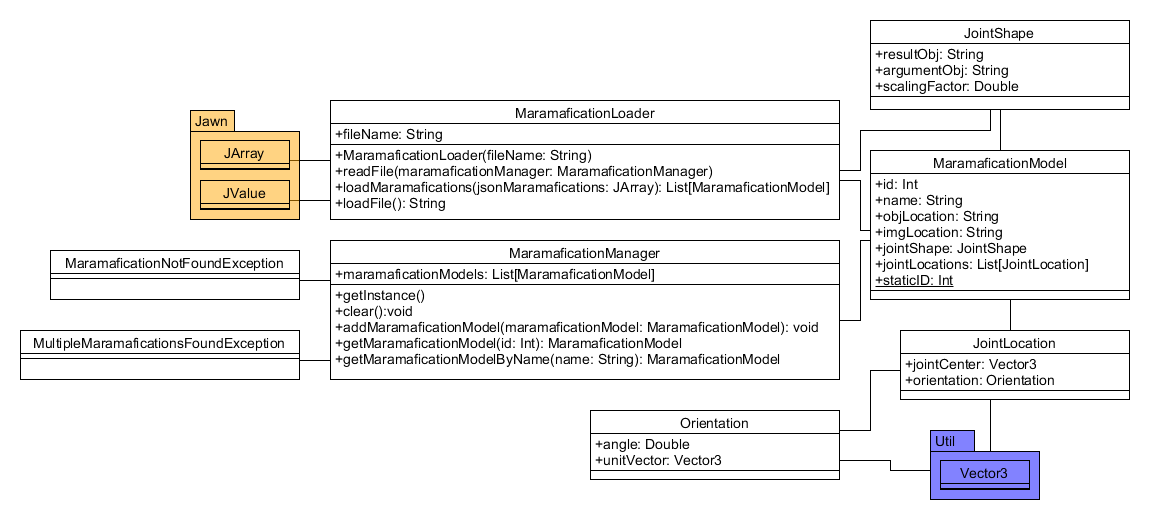
\includegraphics[width=\textwidth, height=\textheight, keepaspectratio]{Marama-Editor}
        \caption{Implementation of the maramafication loader and storing the maramafications}
    \end{figure}
    More information about the reasoning behind this particular structure is found inside the Design Choices\ref{sec:designchoices} section.
    In this section the communication flow of the loader is explained.
    This contains an explanation of how a JSON file gets parsed into a list of MaramaficationModels.

    From the main thread the MaramaficationLoader will be created, passing through the file (.mar) that has to be read.
    After that the \textit{readFile()} method is called.
    This will respectively call the \textit{loadFile()} and the \textit{loadMaramafications()} methods.
    A string is constructed first, which contains all the data of the file.
    Implying this file meets the standards, there will be a list of MaramaficationModels in JSON format.
    There will also be the JointLocations and a JointShape needed to construct these MaramaficationModels.
    Then, the Jawn library is used to parse the string. Due to the file being a list of MaramaficationModels, a JArray will be passed through the \textit{loadMaramafications()} method.
    \newpage
    \begin{figure}[htb]
        \center
        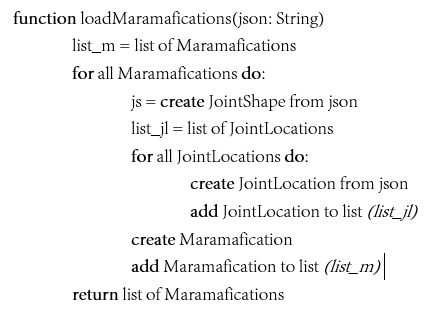
\includegraphics[width=60mm, keepaspectratio]{pseudocode}
        \caption{Pseudocode of the \textit{loadMaramafications()} method}
    \end{figure}

    The above pseudocode gives an idea of how the loadMaramafications method works.
    The list of Maramafications will finally be loaded inside the MaramaficationManager and the job is done.
    The MaramaficationManager being a singleton makes it accessible from the whole application, always being able to fetch the loaded MaramaficationModels.

    \subsection{Project Structure}
    Artifacts are built using sbt by passing the correct arguments, like so: \texttt{sbt assembly}.
    Sbt also manages the dependencies of the project.
    Next up is the documentation directory which, together with a local auxil directory make up our documentation, using \LaTeX\ of course.
    Finally there are a couple of build and property files together with the gitignore file.

    \newpage

    %------------------------------------------------------------------------------------------------------------------------------------------------------- Design Choices
    \section{Design Choices}
    \label{sec:designchoices}

    First a design has been made for the editor as a whole.
    Note that this is loosely based on UML but does not follow a specific UML standard.
    Furthermore it does not denote any concrete implementation.\\
    \begin{figure}[htb]
        \centering
        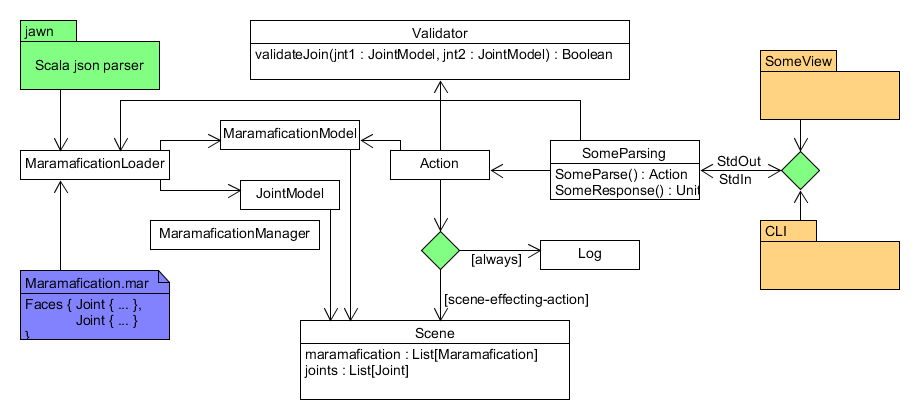
\includegraphics[width=\textwidth, height=\textheight, keepaspectratio]{architecture-marama-editor}
        \caption{The overview diagram of the marama-editor, used as blueprint in the early stages of development}
        \label{fig:ame}
    \end{figure}
    Figure \ref{fig:ame} shows the first prototype of the editor project.
    The idea was that the marama-editor would be a stand-alone terminal based program.
    This way it is easy for a seperate GUI project to attach itself to the editor, redirecting input and visualizing the state of the marama-editor.
    Now we encounter the entry point of the program.
    First some parsing has to be done, it looks for legal commands and fires the appropriate action(s), see:\ref{itm:actions}.
    The fired action will then either load a .mar file with the \code{MaramaficationLoader}, adding it to the Scene via the \code{MaramaficationManager}.
    The \code{MaramaficationLoader} parses .mar files to the internal structure of the \code{MaramficationModel} and the \code{JointModel}.
    The \code{MaramaficationManager} manages all loaded \code{MaramficationModel} s and \code{JointModel} s.
    The \code{Scene} tracks all instantiated \code{MaramficationModel} s and \code{JointModel} s.
    All \code{Actions} should be logged, as this is a requirement from the product owner.
    Other actions like clicking and selecting different maramafication in the view should be logged by the marama-editor.
    Finally there is the \code{Validator} that validates if two \code{MaramaficationModels} are allowed to be joined.

    The various actions are:
    \begin{description}
        \label{itm:actions}
        \item[Concrete actions]: actions that do modify the \code{Scene}
        \begin{description}
            \item[load] Loads a .mar file
            \item[add] Adds a instance of a \code{MaramaficationModel} to the \code{Scene}
            \item[join] Validate two \code{MaramaficationModel} instances
            \item[log] Log another \code{Action}
            \item[delete] Delete a \code{MaramaficationModel} instance from the \code{Scene}
            \item[clear] Deletes all \code{MaramaficationModel} instances from the \code{Scene}
        \end{description}
        \item[User actions]: actions that do not modify the \code{Scene} and should only be logged
        \begin{description}
            \item[select from list] User selected a \code{MaramaficationModel} from the palette.
            \item[select in scene] User selected an instantiated \code{MaramaficationModel}
            \item[move maramafication] User moved a instantiated \code{MaramaficationModel}
        \end{description}
    \end{description}

    \subsection{Joints, Models and Instances}
    \label{sec:marama-storage}
    This section will explain the way the marama logic has taken shape implemented in code.\\
    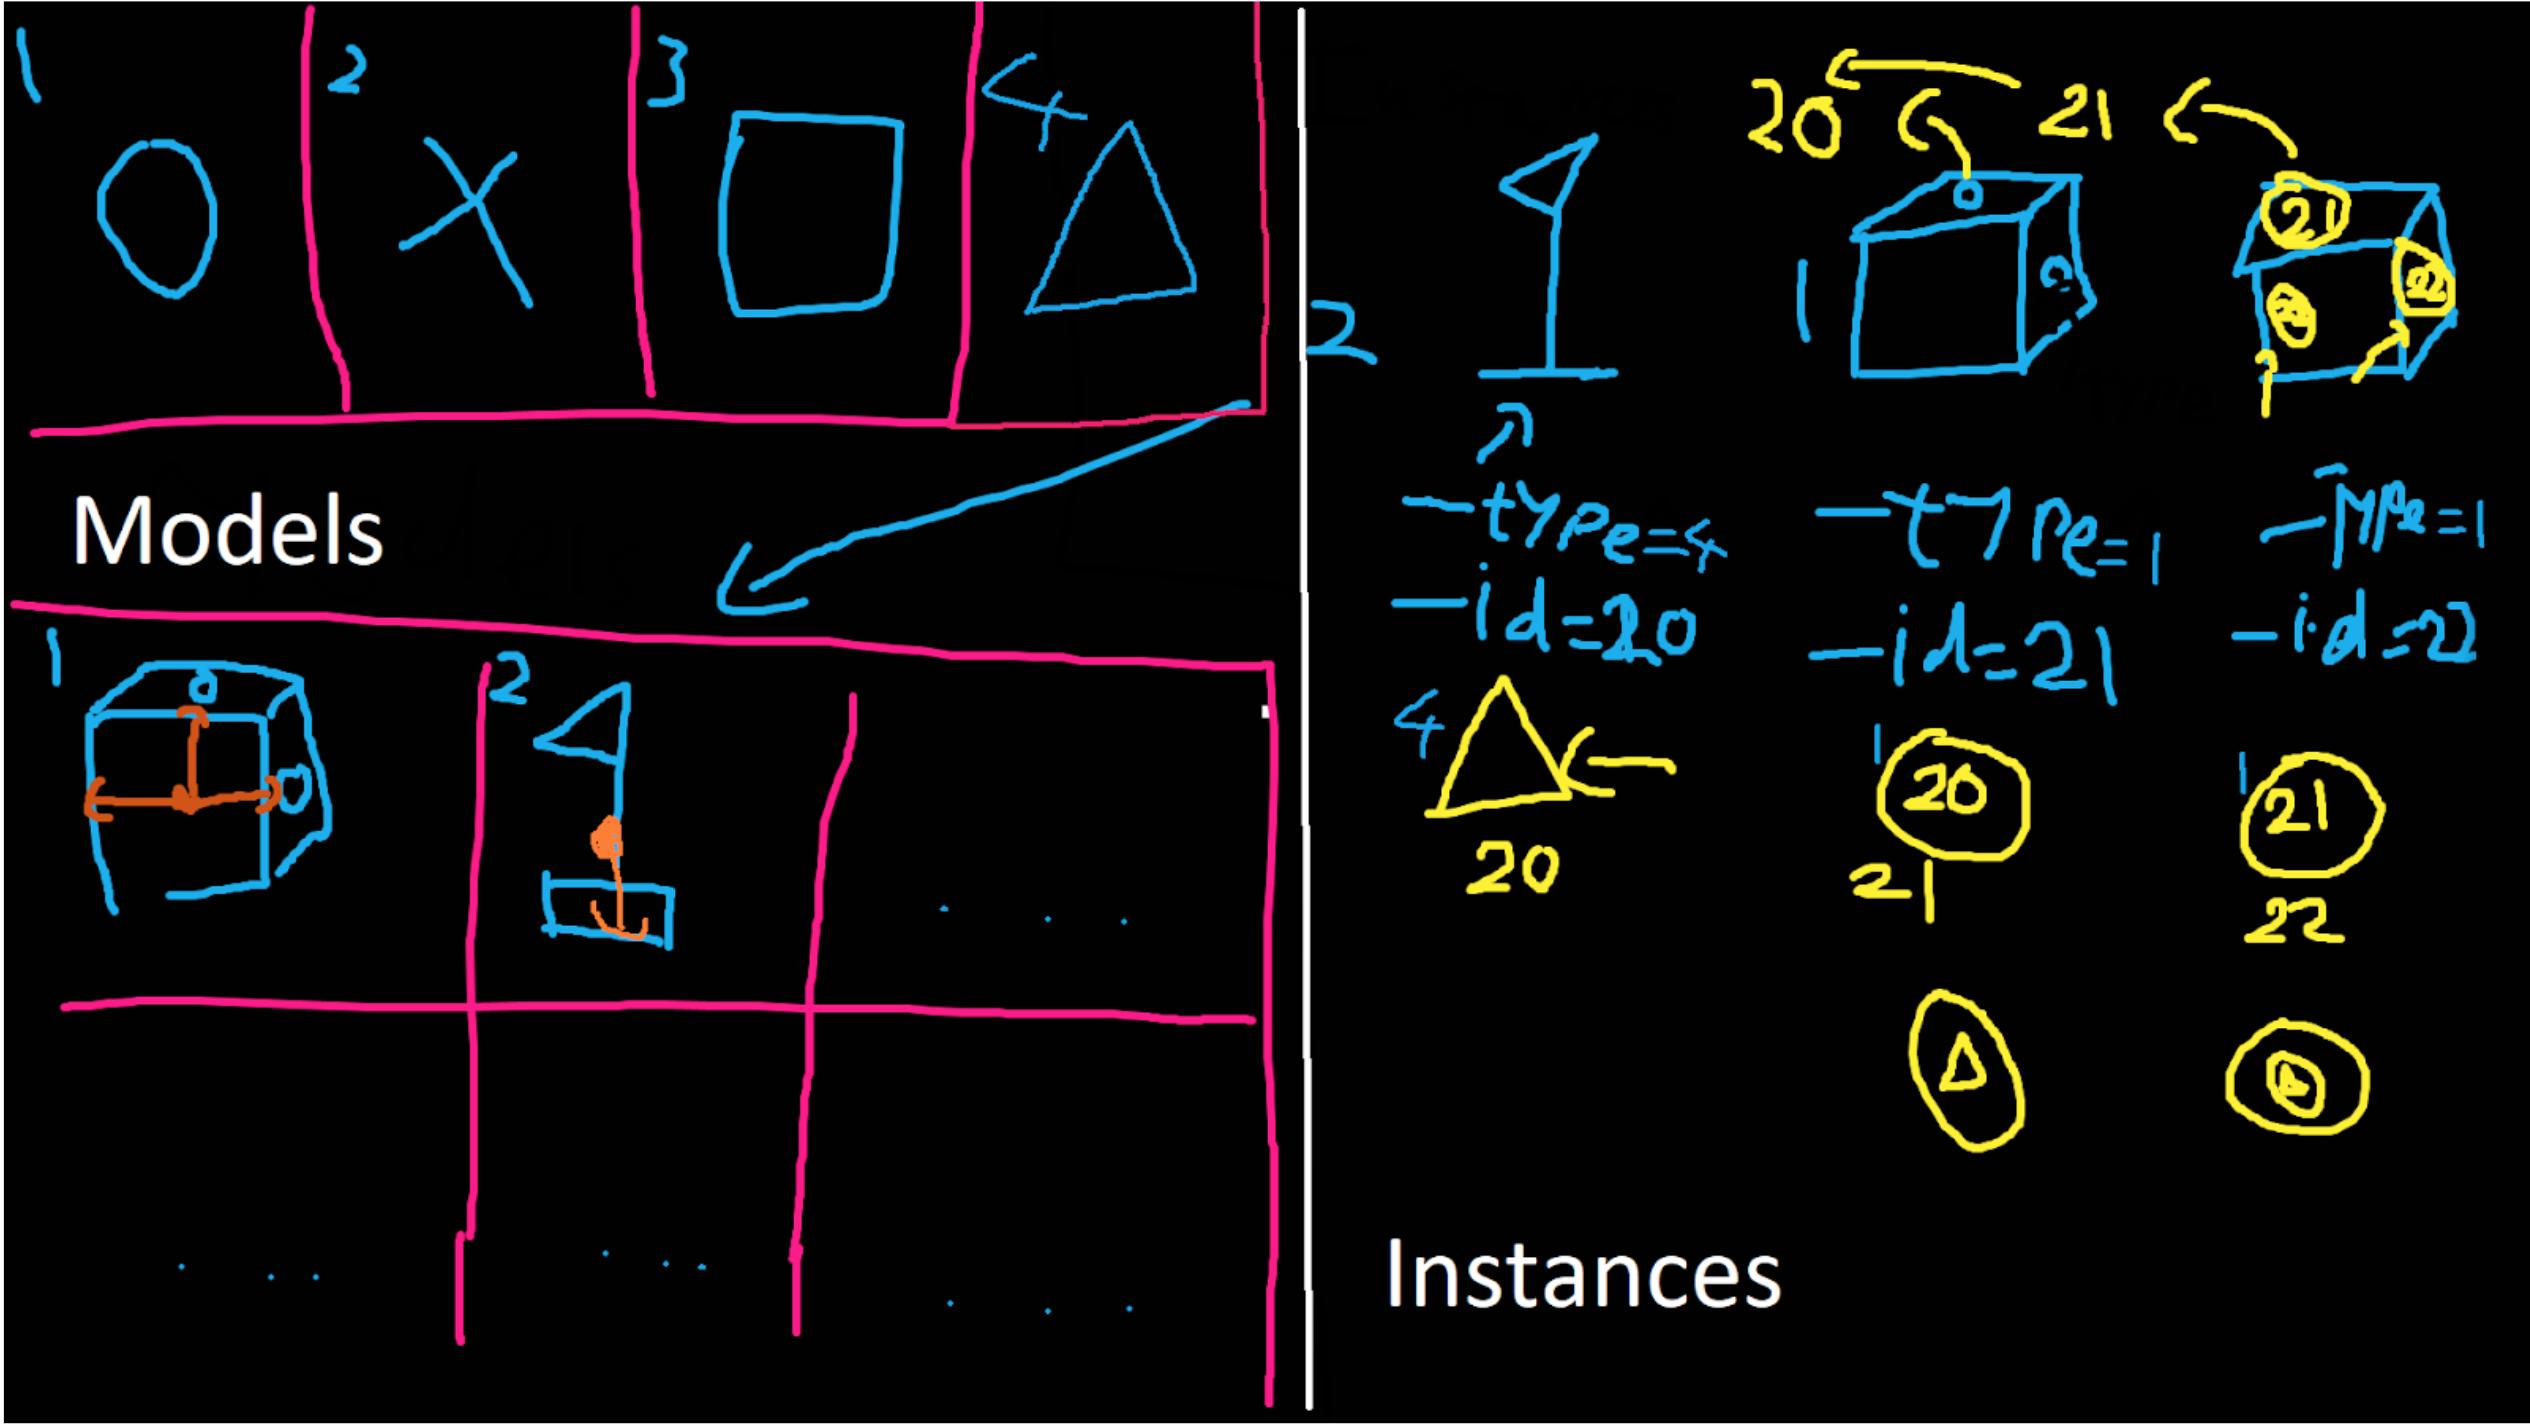
\includegraphics[width=1\linewidth]{marama-joins-models-instances.png}

    The image above is divided in three parts: the joints (top-left), the models (bottom-left) and the instances (right).
    A joint is a shape that can be attached to a single face of a model.
    Every joint has a unique type-id that is used as a reference to this joint.
    When a joint is added to a model, this combination can be seen as an instance.
    The joint will decide whether another instance will fit on this model.

    When the user tries to build a marama (a combination of instances) the user will always try to fit instances together.
    Every instance has a unique id, a number that is used as a reference to this instance.
    Besides the id, the instance also contains info about his faces and the possible joints that are attached.
    When two instances are connected, the facing joints will be checked if they fit.
    Joints can connect if they are of the same type-id and when they differ in gender, either male or female.
    If this is the case, both instances will receive a reference to each other.
    This reference will tell whether the instances are connected or not, and to what.
    \subsection[Communication MVA-MEA]{Receiving command or information from MVA and MEA}
    \label{subsec:comchoice}
    In the ideal situation the Editor would be a command line tool for the Marama project.
    This way, it is easy to build a different, or more specialized view on top of the Editor.

    \subsection{Epics}
    \label{subsec:epics}
    The editor is made up of different epics.\\
    Epics are a collection of user stories that share a goal or functionality.

    \newcommand{\clickup}[1]{https://app.clickup.com/757520/761304/t/#1}

    \myparagraph{\href{\clickup{2e28f}}{\#2e28f} As a MD I want my maramafications to be added to the list inside the Marama-editor (loading .obj files)}
    A lot of the implementation of this user story depended on the data we received from the transpiler (a piece of code constructing the .mar files).
    Since the transpiler isn't finished yet, all needed information could be made available.
    This information should be based on the visupol.pdf\cite{visupol} paper.
    Then of course, the properties of the classes stored inside the MaramaficationManager are based on the contents of this same paper as well.

    A .mar file is constructed according to the specifications of this paper.
    This file is used for testing purposes, and the code of the MaramaficationLoader is built around it.
    The loaders expects the file to meet the following requirements:

    \begin{description}
        \item[MaramaficationModels] A list of MaramaficationModels
        \begin{description}
            \item[Name] Textual identification
            \item[ObjLocation] 3D object location
            \item[ImageLocation] Preview image location
            \item[JointShape] Maramafication specific joint shape
            \begin{description}
                \item[Argument] Argument 3D object location
                \item[Result] Result 3D object location
                \item[ScalingFactor] Factor for object scaling
            \end{description}
            \item[JointLocations] List of all JointLocations
            \begin{description}
                \item[JointCenter] Vector3 defining the position of the joint
                \begin{description}
                    \item[X, Y, Z]
                \end{description}
                \item[Orientation] Direction the joint is facing
                \begin{description}
                    \item[Angle] Rotation of the joint
                    \item[UnitVector] Vector3 defining the direction
                    \begin{description}
                        \item[X, Y, Z]
                    \end{description}
                \end{description}
            \end{description}
        \end{description}
        \item
    \end{description}

    The received JSON is getting parsed.
    To do this we chose the \href{https://github.com/non/jawn}{Jawn library}.
    Scala doesn't support JSON parsing natively, which forced to use a library.
    The chosen library is Jawn, it gets the job done without being overly complicated.

    \newpage
    %------------------------------------------------------------------------------------------------------------------------------------------------------- Build Automation
    \section{Continous Integration}
    In this section build automation and its constituent components will be discussed.
    How we applied it, the software used and the targets and platforms supported are among a few.

    The requirements for the project contain several important matters.
    The project needs to be able to be developed and built from all OSes.
    It needs to be able to switch hands between multiple developers easily, due to it being open source.
    It should also obviously be thoroughly tested.
    Because of this, the team, together with Chide decided that a continuous integration solution was necessary, and have been working on setting this up during the first part of the project.

    The chosen CI system is Travis CI .
    It is free for open source, and easy to use and learn.
    After some research between multiple options the available documentation, resources, and functionality, such as the multi-os build options, made the team decide that Travis would be the best option.
    There were a few problems with the setup, which will be detailed further below.
    The current implementation of Travis CI:
    \begin{itemize}
                 \item-Sets up a container for the project to run.
                 \item-Automatically builds the project
                 \item-Runs through all unit tests
                 \item-Allows live views and checks of the build.
             \end{itemize}
    This is currently always a Linux build, due to being unable to properly set up a Mac OS or Windows build.
    This ensures that all commits have been properly tested.
    Code review can be done without having to clone and test the code yourself.
    +
    \textbf{Notes on Travis setup:}
    Travis needs to be activated per repository.
    The team repository has it activated, but that permission won't come along when it is merged to the main branch.
    To activate this you will need to go to the travis website and allow them access to your GitHub account, then toggle the repositories you want it to review.
    %------------------------------------------------------------------------------------------------------------------------------------------------------- Continuing Development
    \section{Continuing Development}
    This section describes the plan on how to continue with development in the best way.
    The team worked on quite some user stories from April 9th, to June 15th.
    The following functionalities are most critical at the moment to start working on:

    \subsection{Instantiating maramafications from a .mar file.}
    A beginning is made at implementing the .mar file.
    The .mar file is, as earlier explained, basically a json file with some agreements on structure.
    The goal of the .mar file is contain data for Maramafications and all that is needed to instantiate one.
    This means that every value from the .mar file is evaluated and constructed into a maramafication model, which is usable in the View.
    This means that it will be placed in the maramafication list of the View.

    \subsection{Consistency according to Visupol}
    Also earlier defined, most of the development is structured according to the visupol\cite{visupol} document.
    However, not everything is consistent yet, and it's advised to first read this article before further developing.
    The inconsistency is explainable by the complexity and the extensiveness of this document.
    It contains the entire concept of Maramafication, including the marama-editor and the marama-view logic, worked out to its full potential.
    Therefore, use this document as a guideline when developing.
    During the developing of the application to its current state, a lot of problems could've been both more quickly and more easily solved if we consulted the visupol article.

    \subsection{Communication from Editor to View}
    The Editor must be able to send its state to the View so the View can visually represent that state.
    This also requires some work inside the View to make this happen.
    The reason behind this is to keep the Editor and View separated.

    \subsection{Saving the state of the View inside the Editor}
    The Editor needs to be able to know the state that the View is in.
    This is because only the Editor is able to know whether a current marama is valid or invalid.
    When something changes in the view, the Editor needs to be able to validate this change and change its state accordingly.
    This is more extensively explained in the design choices\cite{sec:marama-storage} section.

    \subsection{Different joint types}
    // TODO: Describe the different joint types and what should be done accordingly


    \newpage
    %------------------------------------------------------------------------------------------------------------------------------------------------------- References
    \bibliography{references}
    \bibliographystyle{ieeetr}
    % options: apalike for apa, ieeetr for ieee
\end{document}
